\begin{comment}
\end{comment}

\chapter{Construction de codes correcteurs quantiques}

Dans le chapitre précédent, 
je me suis intéressé à la correction des erreurs lors de la communication classique.
Pour la suite de la thèse,
je quitterai ce régime pour m'intéresser au régime quantique.
Dans ce chapitre, 
je m'intéresserai plus particulièrement à la protection de l'information 
dans un modèle quantique simplifié avant de présenter la conception d'une mémoire 
quantique au prochain chapitre.
Ce modèle simplifié ressemble au canal binaire symétrique présenté au premier chapitre
et il permet d'étudier la construction de codes correcteurs d'erreurs quantiques sans prendre en compte les détails d'implémentation.

De façon semblable au scénario classique,
concevoir des codes correcteurs qui permettent de bien protéger l'information avec un nombre raisonnable de qubits supplémentaires est crucial.
En fait,
la présence des erreurs est l'un des obstacles parmi les plus
limitants pour la réalisation de calculs quantiques.
Ainsi, 
la correction d'erreurs ne se limite pas à des scénarios de communication 
comme dans le cas classique,
mais sera omniprésente dans un système de calcul quantique.

Cette importance accrue des erreurs dans les systèmes quantiques s'explique
principalement du fait qu'il s'agit de systèmes analogues plutôt que digitaux.
Un système est digital lorsque chacun de ses éléments peut prendre un nombre fini
de valeurs. 
Dans le cas des ordinateurs classiques,
chaque bit prend soit la valeur 0 ou la valeur 1.
Ainsi,
une quantité continue comme une différence de potentiel représente physiquement un bit tout en le protégeant des erreurs.
Par exemple,
le bit 0 peut être associé à une valeur de 0 volt et le bit 1 à une valeur de 5 volts.
Dans le cas où une valeur de 4.9 volts serait mesurée, il est fort probable que 
la valeur désirée soit le bit 1.
Donc, en absence des perturbations externes présentent lors de la communication,
l'information classique est relativement robuste.

Au contraire, un système quantique est analogue puisqu'il existe une infinité d'états accessibles.
Par exemple, deux nombres complexes $a$ et $b$ avec la seule contrainte que $a^2 + b^2 = 1$ représente l'état d'un qubit. 
Une faible variation de ces paramètres représente un état différent.
Savoir si l'état du système est l'état désiré ou un état corrompu est généralement impossible.
De plus, l'accumulation de petites différences sur l'état de chaque bit peut complètement
changer le résultat d'un calcul.

Ces erreurs émergent généralement de processus de décohérence.
Par exemple,
un système quantique dans un état excité tend naturellement à retourner dans un état de moindre énergie.
Au milieu des années 1990,
plusieurs scientifiques croyaient que
les erreurs engendrées par la décohérence des systèmes quantiques
représentaient un obstacle insurmontable au calcul quantique~\cite{unruh_maintaining_1995, palma_quantum_1996, landauer_is_1995, chuang_quantum_1995}.
Leurs arguments reposaient entre autres sur le théorème de non-clonage~\cite{wootters_single_1982}
stipulant qu'il est impossible de copier l'état d'un qubit vers un second qubit.
Cela semblait donc empêcher l'utilisation de la redondance pour 
protéger le système des erreurs comme c'est le cas pour la communication classique.

Nous savons aujourd'hui comment contourner ces limitations. 
Les premiers à avoir proposé une solution sont Calderbank, Shor et Steane~\cite{calderbank_good_1996, steane_multiple-particle_nodate}.
D'ailleurs, à la prochaine section,
je vais introduire une importante famille de codes correcteurs quantiques, les codes CSS, qui porte leur nom.
En réponse à ce résultat, Gottesman~\cite{gottesman_stabilizer_1997} a introduit le formalisme des codes stabilisateurs
que je vais utiliser dans ce chapitre pour décrire les codes correcteurs quantiques.

Depuis,
plusieurs familles de codes correcteurs quantiques ont été introduites.
Les codes les plus étudiés sont sans aucun doute les codes de surfaces et 
les codes toriques introduits par Kitaev~\cite{kitaev_fault-tolerant_2003}.
Cependant,
ces codes, bien qu'excellent pour protéger le système,
ne permettent pas d'encoder efficacement un grand nombre de qubits~\cite{bravyi_tradeoffs_2010}.
Pour contrer ce problème,
les codes quantiques d'opérateurs de parité à faible 
densité~(LDPC, de l'anglais \textit{low-density parity-check})
reçoivent de plus en plus d'attention.
Les codes quantiques LDPC incluent plusieurs familles,
dont les codes par produit d'hypergraphes~\cite{tillich_quantum_2014}
et les codes par produit homologique~\cite{bravyi_homological_2014}.

Comme leur nom l'indique,
les codes quantiques LDPC sont généralement obtenus par le produit 
de structures associées à des codes correcteurs classiques.
Dans le cadre de cette thèse,
j'ai conçu une approche qui permet de générer des codes correcteurs quantiques
directement,
sans avoir recours à une construction classique au préalable.
L'un des principaux avantages de cette méthode est sa flexibilité 
lors de la construction des codes.
De plus,
elle permet d'identifier des régimes pour lesquels il est aisé de
construire des codes correcteurs quantiques
et des régimes pour lesquels la tâche est beaucoup plus ardue.

Dans ce chapitre,
je présenterai les notions essentielles pour bien comprendre ce résultat.
D'abord,
je présenterai le formaliste des codes stabilisateurs
avant d'introduire les problèmes de satisfaction de contraintes sur lesquels 
se base ma construction de codes.
Finalement,
je présenterai l'article expliquant la construction et 
mettant de l'avant les résultats de ce projet.

\section{Codes stabilisateurs et correction d'erreurs quantique}
\subsection{Théorème du seuil et évaluation de la performance des codes correcteurs quantiques}

\section{Problèmes de satisfaction de contraintes}

\section{Article : Une multitude de codes stabilisateurs éparses}

Cet article soumis au journal Quantum à l'été 2022 a pour titre original \textit{Finite-rate quantum sparse codes aplenty}.
Celui-ci était toujours en processus de révision lors de la soumission de cette thèse.

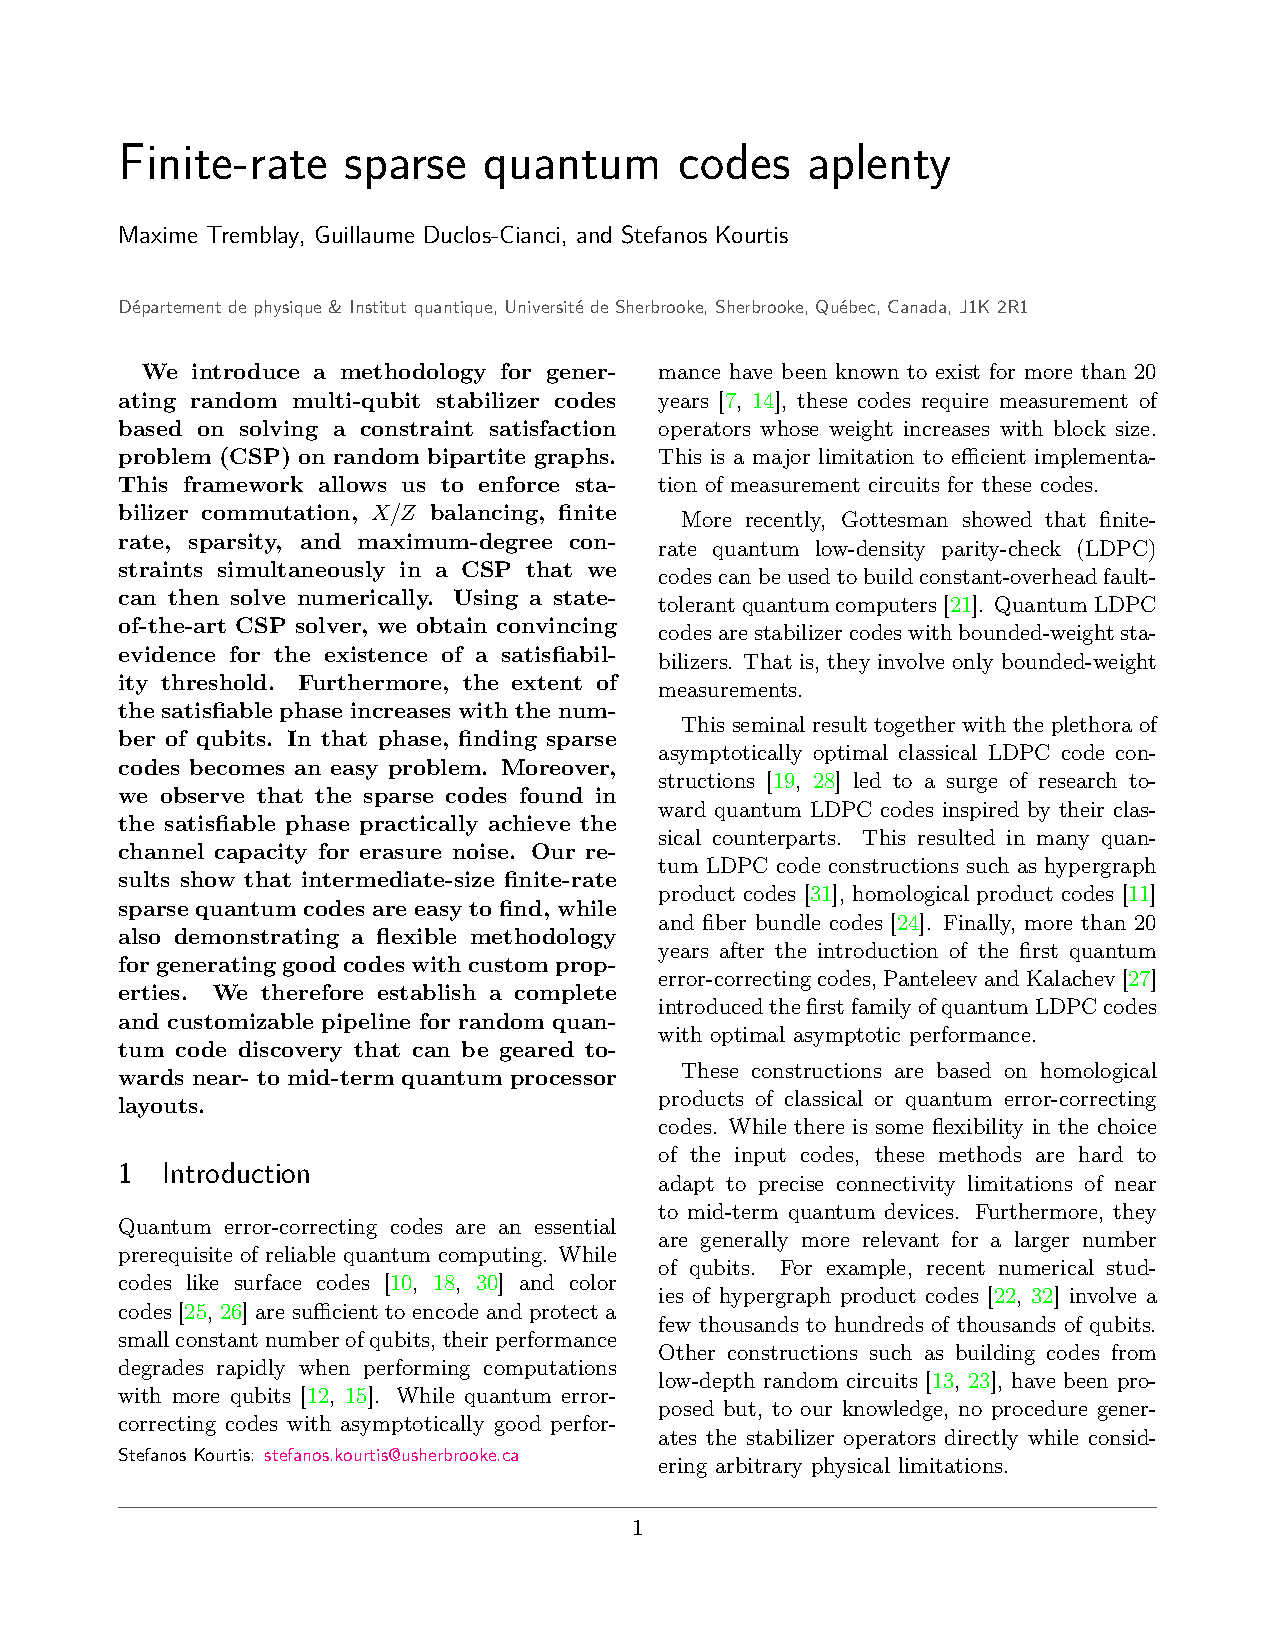
\includepdf[pages=-]{articles/sat_codes_construction.pdf}
